% GNUPLOT: LaTeX picture with Postscript
\begingroup
  \makeatletter
  \providecommand\color[2][]{%
    \GenericError{(gnuplot) \space\space\space\@spaces}{%
      Package color not loaded in conjunction with
      terminal option `colourtext'%
    }{See the gnuplot documentation for explanation.%
    }{Either use 'blacktext' in gnuplot or load the package
      color.sty in LaTeX.}%
    \renewcommand\color[2][]{}%
  }%
  \providecommand\includegraphics[2][]{%
    \GenericError{(gnuplot) \space\space\space\@spaces}{%
      Package graphicx or graphics not loaded%
    }{See the gnuplot documentation for explanation.%
    }{The gnuplot epslatex terminal needs graphicx.sty or graphics.sty.}%
    \renewcommand\includegraphics[2][]{}%
  }%
  \providecommand\rotatebox[2]{#2}%
  \@ifundefined{ifGPcolor}{%
    \newif\ifGPcolor
    \GPcolortrue
  }{}%
  \@ifundefined{ifGPblacktext}{%
    \newif\ifGPblacktext
    \GPblacktexttrue
  }{}%
  % define a \g@addto@macro without @ in the name:
  \let\gplgaddtomacro\g@addto@macro
  % define empty templates for all commands taking text:
  \gdef\gplbacktext{}%
  \gdef\gplfronttext{}%
  \makeatother
  \ifGPblacktext
    % no textcolor at all
    \def\colorrgb#1{}%
    \def\colorgray#1{}%
  \else
    % gray or color?
    \ifGPcolor
      \def\colorrgb#1{\color[rgb]{#1}}%
      \def\colorgray#1{\color[gray]{#1}}%
      \expandafter\def\csname LTw\endcsname{\color{white}}%
      \expandafter\def\csname LTb\endcsname{\color{black}}%
      \expandafter\def\csname LTa\endcsname{\color{black}}%
      \expandafter\def\csname LT0\endcsname{\color[rgb]{1,0,0}}%
      \expandafter\def\csname LT1\endcsname{\color[rgb]{0,1,0}}%
      \expandafter\def\csname LT2\endcsname{\color[rgb]{0,0,1}}%
      \expandafter\def\csname LT3\endcsname{\color[rgb]{1,0,1}}%
      \expandafter\def\csname LT4\endcsname{\color[rgb]{0,1,1}}%
      \expandafter\def\csname LT5\endcsname{\color[rgb]{1,1,0}}%
      \expandafter\def\csname LT6\endcsname{\color[rgb]{0,0,0}}%
      \expandafter\def\csname LT7\endcsname{\color[rgb]{1,0.3,0}}%
      \expandafter\def\csname LT8\endcsname{\color[rgb]{0.5,0.5,0.5}}%
    \else
      % gray
      \def\colorrgb#1{\color{black}}%
      \def\colorgray#1{\color[gray]{#1}}%
      \expandafter\def\csname LTw\endcsname{\color{white}}%
      \expandafter\def\csname LTb\endcsname{\color{black}}%
      \expandafter\def\csname LTa\endcsname{\color{black}}%
      \expandafter\def\csname LT0\endcsname{\color{black}}%
      \expandafter\def\csname LT1\endcsname{\color{black}}%
      \expandafter\def\csname LT2\endcsname{\color{black}}%
      \expandafter\def\csname LT3\endcsname{\color{black}}%
      \expandafter\def\csname LT4\endcsname{\color{black}}%
      \expandafter\def\csname LT5\endcsname{\color{black}}%
      \expandafter\def\csname LT6\endcsname{\color{black}}%
      \expandafter\def\csname LT7\endcsname{\color{black}}%
      \expandafter\def\csname LT8\endcsname{\color{black}}%
    \fi
  \fi
  \setlength{\unitlength}{0.0500bp}%
  \begin{picture}(7936.00,3968.00)%
    \gplgaddtomacro\gplbacktext{%
      \csname LTb\endcsname%
      \put(980,640){\makebox(0,0)[r]{\strut{} 0}}%
      \put(980,1005){\makebox(0,0)[r]{\strut{} 200}}%
      \put(980,1370){\makebox(0,0)[r]{\strut{} 400}}%
      \put(980,1736){\makebox(0,0)[r]{\strut{} 600}}%
      \put(980,2101){\makebox(0,0)[r]{\strut{} 800}}%
      \put(980,2466){\makebox(0,0)[r]{\strut{} 1000}}%
      \put(980,2831){\makebox(0,0)[r]{\strut{} 1200}}%
      \put(980,3197){\makebox(0,0)[r]{\strut{} 1400}}%
      \put(980,3562){\makebox(0,0)[r]{\strut{} 1600}}%
      \put(980,3927){\makebox(0,0)[r]{\strut{} 1800}}%
      \put(1100,440){\makebox(0,0){\strut{}361.645650}}%
      \put(2179,440){\makebox(0,0){\strut{}361.645700}}%
      \put(3258,440){\makebox(0,0){\strut{}361.645750}}%
      \put(4337,440){\makebox(0,0){\strut{}361.645800}}%
      \put(5417,440){\makebox(0,0){\strut{}361.645850}}%
      \put(6496,440){\makebox(0,0){\strut{}361.645900}}%
      \put(7575,440){\makebox(0,0){\strut{}361.645950}}%
      \put(160,2283){\rotatebox{-270}{\makebox(0,0){\strut{}Countrate [s$^{-1}$]}}}%
      \put(4337,140){\makebox(0,0){\strut{}Frequenz [THz]}}%
      \put(1294,3598){\makebox(0,0)[l]{\strut{}$G(\nu)=A\cdot\frac{1}{\sigma\sqrt{2\pi}}\mathrm{e}^{-\frac{1}{2}\frac{(\nu-\mu)^2}{\sigma^2}}+b$}}%
      \put(1294,3105){\makebox(0,0)[l]{\strut{}$2\sigma = (26.64\pm0.52)\,$MHz}}%
      \put(1294,2875){\makebox(0,0)[l]{\strut{}$\mu = (361.64583384\pm0.00000022)\,$THz}}%
      \put(1294,2645){\makebox(0,0)[l]{\strut{}$A = (0.0541\pm0.0011)\,\nicefrac{\text{MHz}}{\text{s}}$}}%
      \put(1294,2415){\makebox(0,0)[l]{\strut{}$b = (30.0\pm9.9)\,$s$^{-1}$}}%
    }%
    \gplgaddtomacro\gplfronttext{%
      \csname LTb\endcsname%
      \put(6672,3764){\makebox(0,0)[r]{\strut{}Messpunkte}}%
      \csname LTb\endcsname%
      \put(6672,3564){\makebox(0,0)[r]{\strut{}Fit}}%
    }%
    \gplbacktext
    \put(0,0){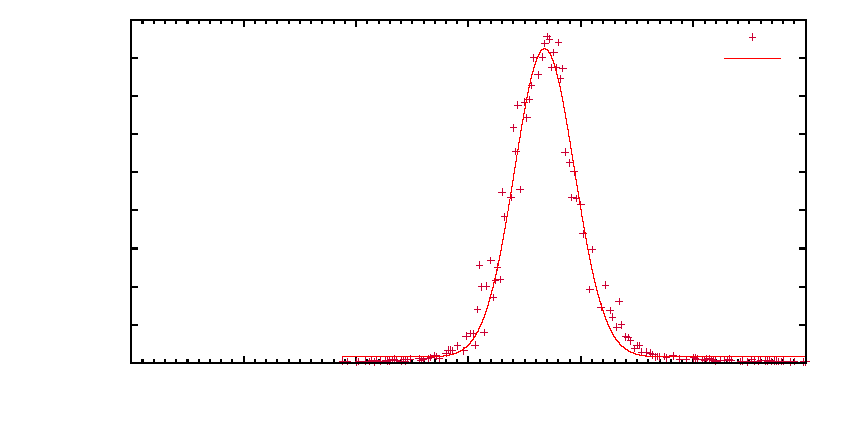
\includegraphics{linienscans_neues_schema_02_SES_mean}}%
    \gplfronttext
  \end{picture}%
\endgroup
